\subsection{Fiducial Cuts}
\label{fidCuts}

Similar to the cuts discussed so far, we also had to match the region of good efficiency of the physical detector with the corresponding region from the simulation. For the experimental and simulation data to be comparable, they must have the same detector acceptance. %, otherwise systematic uncertainty is introduced into the calculations. 
Two event variables polar angle (\thvtx) measured at the vertex and the azimuthal angle $\phi_{DC1}$ measured at the drift chamber layer 1 are chosen to define the good efficiency regions of the detector. The reason for the choice of the variable \thvtx should be obvious because it is directly related with the kinematic variables \qsqs and $W$ used in the analysis. However, due to the momentum dependent rotational effect of the magnetic field on the reconstructed azimuthal angle (\phvtx) at the vertex, the angle $\phi_{DC1}$ is preferred over \phvtx to define the fiducial region because that allows the easy selection (rejection) of the events which passed through and got detected by the more (less) reliable central (marginal) regions of the Cerenkov Counters. %drift chambers. %kp: 12/6/13 after SEK insistence
After a careful and extensive study of the event distributions on both data and simulation, we arrived at four sets of fiducial cuts in terms of the variables \thvtx, $\phi_{DC1}$ and the torus current normalized inverse momentum i.e., \invP.%I$_{torus}$/2250p.% This cut allowed the maximum possible inclusion of the high efficiency regions of

%
% Pass2 fiducial cuts: all defined in #include "/home/adhikari/LinkedFiles/fiducialCutsPass2.h"   
% The final results were for array indices C71 and S181
% The fiducial cuts used for C71_S181 were
%   
%
%   fidCtV1 
%   fidCtExpBySimAndEConlyInInvPvsThVtx
%   fidMoreMIPB
%
% %%%%%%%%%%%%%%%%  
%
%  where,
%   fidCtV1: if(fidCtExp2Sim==true && fidCtReg2EC==true) fidCtV1 = true;
%       with
%  bool fidCtReg2EC = Pass2FidCutLatestFromRegECcomparison(Ebi, p[0], thDc1PosRad);//now in the same fiducialCutsPass2.h file
%     corresponding image: 
%           https://www.jlab.org/Hall-B//secure/eg4/adhikari/Analysis/Pass2/Cuts/Fid/BkUp/invMomVsThDc1Pass2Ebi4Ratio.gif
%
%  bool fidCtExp2Sim = Pass2FidCutLatest(phDc1PosRad, thetaRadC); //now in the same fiducialCutsPass2.h file
%    corresponding image:
%          https://www.jlab.org/Hall-B//secure/eg4/adhikari/Analysis/Pass2/Cuts/Fid/fidCutPlotsSet2_Eb2_RatioBigger.gif 
%          &.../fidCutPlotsSet2_Eb1_Ratio.gif
%
%   
%
%   fidCtExpBySimAndEConlyInInvPvsThVtx = Pass2FidCutOnInvPvsThVtx(Ebi, ppC, thetaRadC);//3/8/16 defined in commonItems4SimExp.h for now
%              ~/secure/Analysis/Pass2/Cuts/Fid/invMomVsThVtxPass2Ebi1RatioRegByEConlyFidCut09.gif
%
%  if(Ebi==2) fidMoreMIPB = moreFidCutsWithMoreInvPBins(Ebi, ppC, phDc1DegPlusMinus30, thVtxDeg);//7/11/16 defined in moreFidCuts.h
%  else if(Ebi==1) fidMoreMIPB = moreFidCutsWithMoreInvPBinsEbi1(Ebi, ppC, phDc1DegPlusMinus30, thVtxDeg);//7/18/16 defined in moreFidCuts.h
%   for which see plots:
%       //https://www.jlab.org/Hall-B//secure/eg4/adhikari/Analysis/Pass2/Cuts/Fid/MoreCts/moreFiducialCutsMoreInversePBinsEbi1.gif
%       and moreFiducialCutsMoreInversePBinsEbi2.gif   //11/13/16
%   




% See EG4 update (Glasgow, by S.E. Kuhn) and make eps plots like those included
% include the DC shadow & granularity  figures, (may be in a separate section on Simulation/GSIM issues and refer to it from this section)

% include the Regular/EC-only 2D plots to show the CC-inefficient regions (to be discarded by some of the angular cuts)
% Show the discrepancy plots in theta and v$_z$ in data and simulation (for a few q2 bins)
%After a laborious work on getting simulation match with the data to a reasonably good degree, we did a final comparison work to determine the fiducial cuts. We obtained overlays of one-dimensional histograms of different variables, and also studied the ratios both in one and two dimensions. Based on these comparisons, regions of relatively bad matching were singled out and cuts were developed to reject such parts of the kinematic space.\textbf{\textcolor{red}{to be be elaborated more ..}}


The first set of fiducial cuts (see Fig. \ref{figFidRegVsEC1}) were determined by comparing regular and EC-only data (which were taken using triggers that didn't involve CC) and selecting cuts such that regions with relatively darker spots (reflecting very low CC-efficiency) were rejected.

\begin{figure}[H]%[h] %ht, htpb (p - float, b = bottom, h=? t = top)
\centering
%\leavevmode 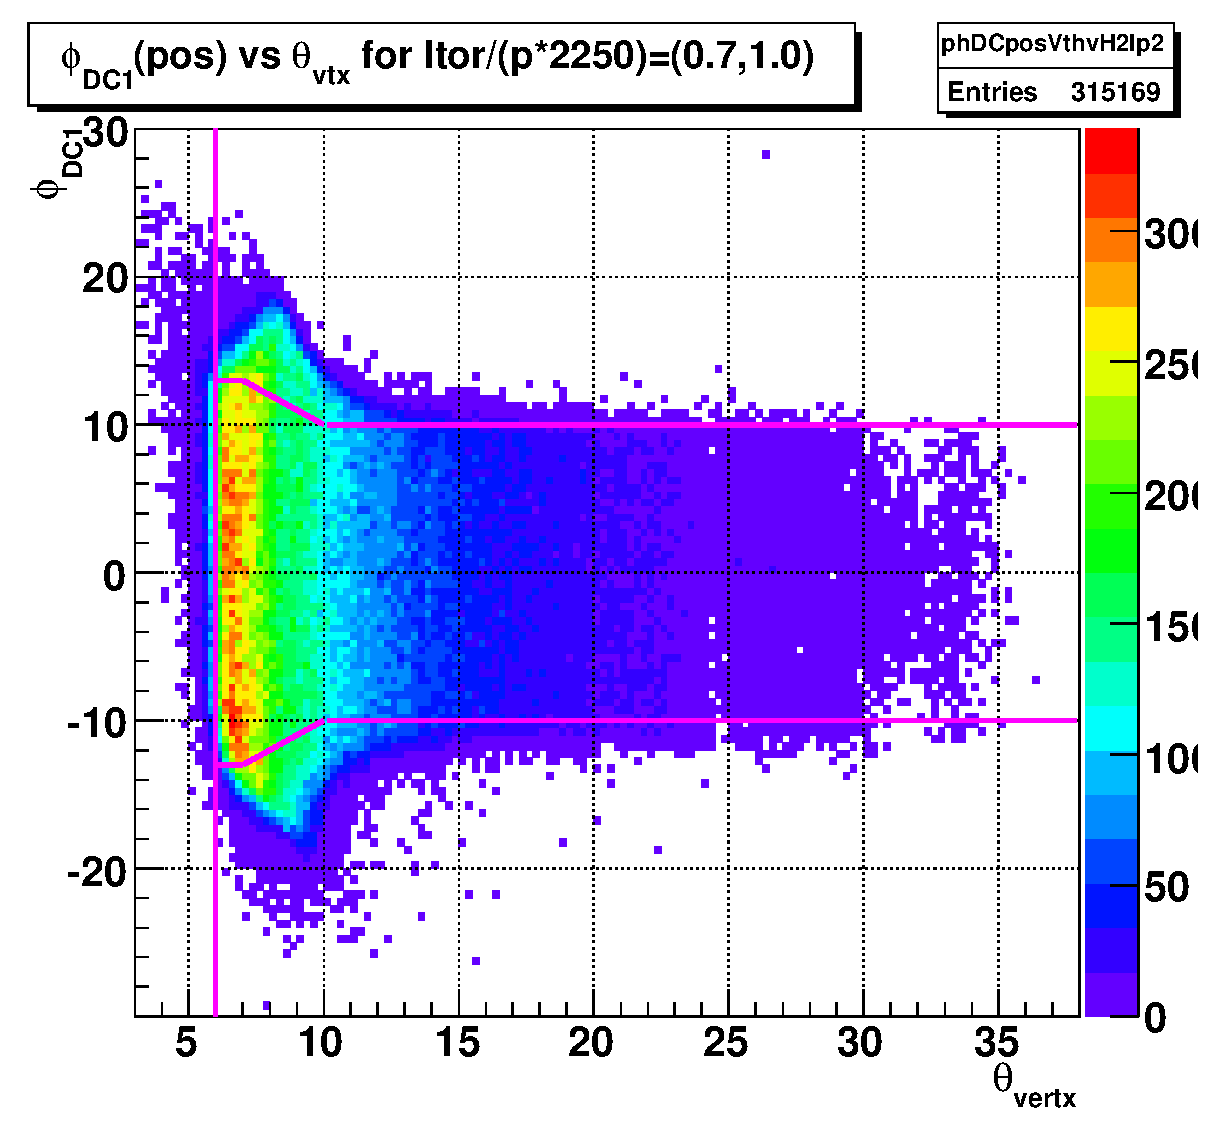
\includegraphics[width=0.9\textwidth]{TexmakerMyFinTh/chap4simul/FigCuts/phDc1PosVsThv_inInvPbins_ExpEb2WdOsiNphNoThCts4Ths.eps} 
%\leavevmode 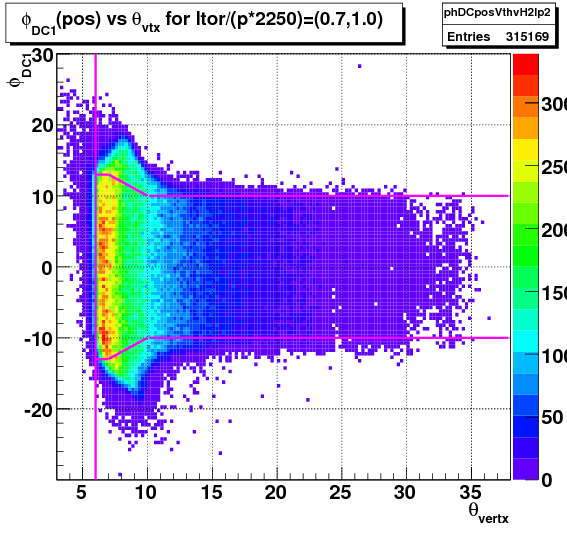
\includegraphics[width=0.9\textwidth]{TexmakerMyFinTh/chap4simul/FigCuts/phDc1PosVsThv_inInvPbins_ExpEb2WdOsiNphNoThCts4Ths} 
%\leavevmode 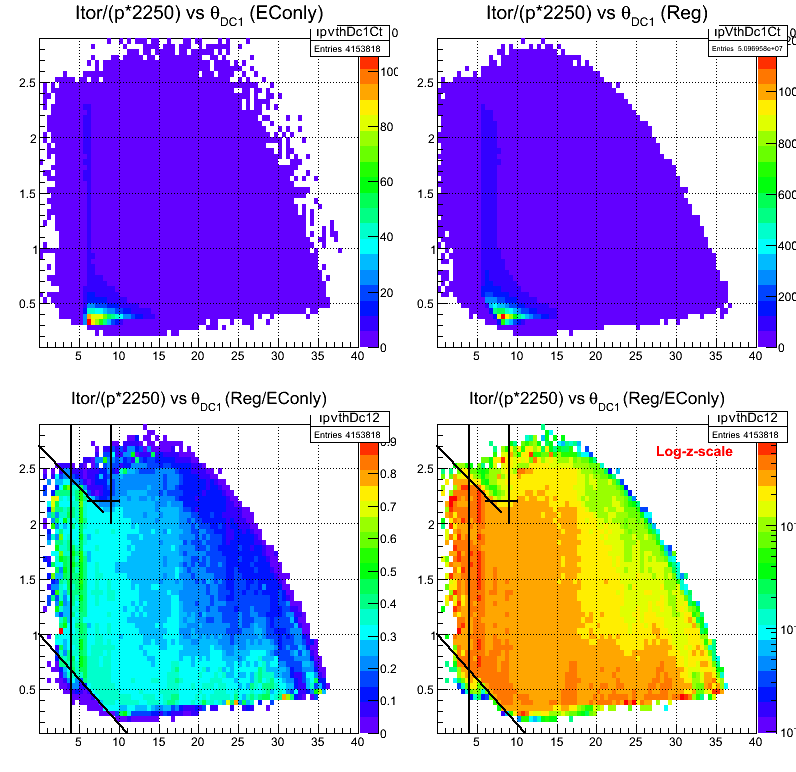
\includegraphics[width=0.9\textwidth]{figuresEG4/NewP2/FidCuts/invMomVsThDc1Pass2Ebi4Ratio.png}
\leavevmode 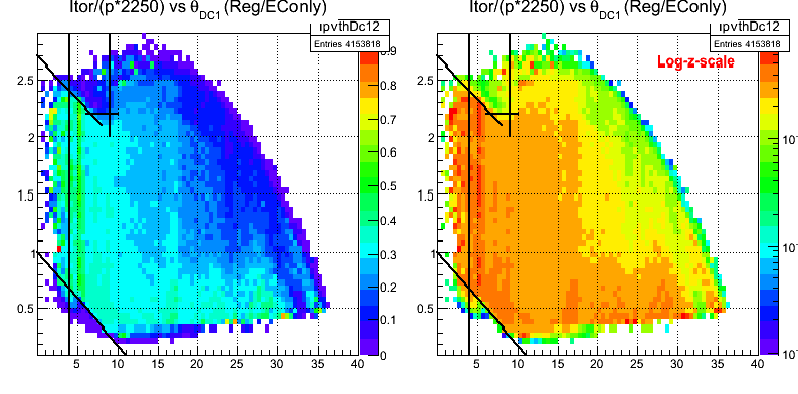
\includegraphics[width=0.9\textwidth]{figuresEG4/NewP2/FidCuts/invMomVsThDc1Pass2Ebi4RatioCropped.png}
\caption[Fiducial cuts]{Fiducial cuts determined by comparing the distributions of regular and EC-only {\bf experimental data} as a function of \invP and $\theta_{DC1}$. %Here in the top panels, we see distributions of regular and EC-only data respectively and in the bottom panel we have the ratios of the two 
Here in the top panels, we see distributions of ratios of the regular and EC-only data respectively in linear and log scales in the color axis respectively. Inefficient regions of the CC are excluded using the indicated cuts.} %Fiducial cuts
\label{figFidRegVsEC1}
\end{figure}

The second set of cuts came from a similar comparison between the regular and EC-only data in the \invP vs \thvtx (instead of $\theta_{DC1}$) space (see Fig. \ref{figFidRegVsEC2}) .

\begin{figure}[H]%[h] %ht, htpb (p - float, b = bottom, h=? t = top)
\centering
%\leavevmode 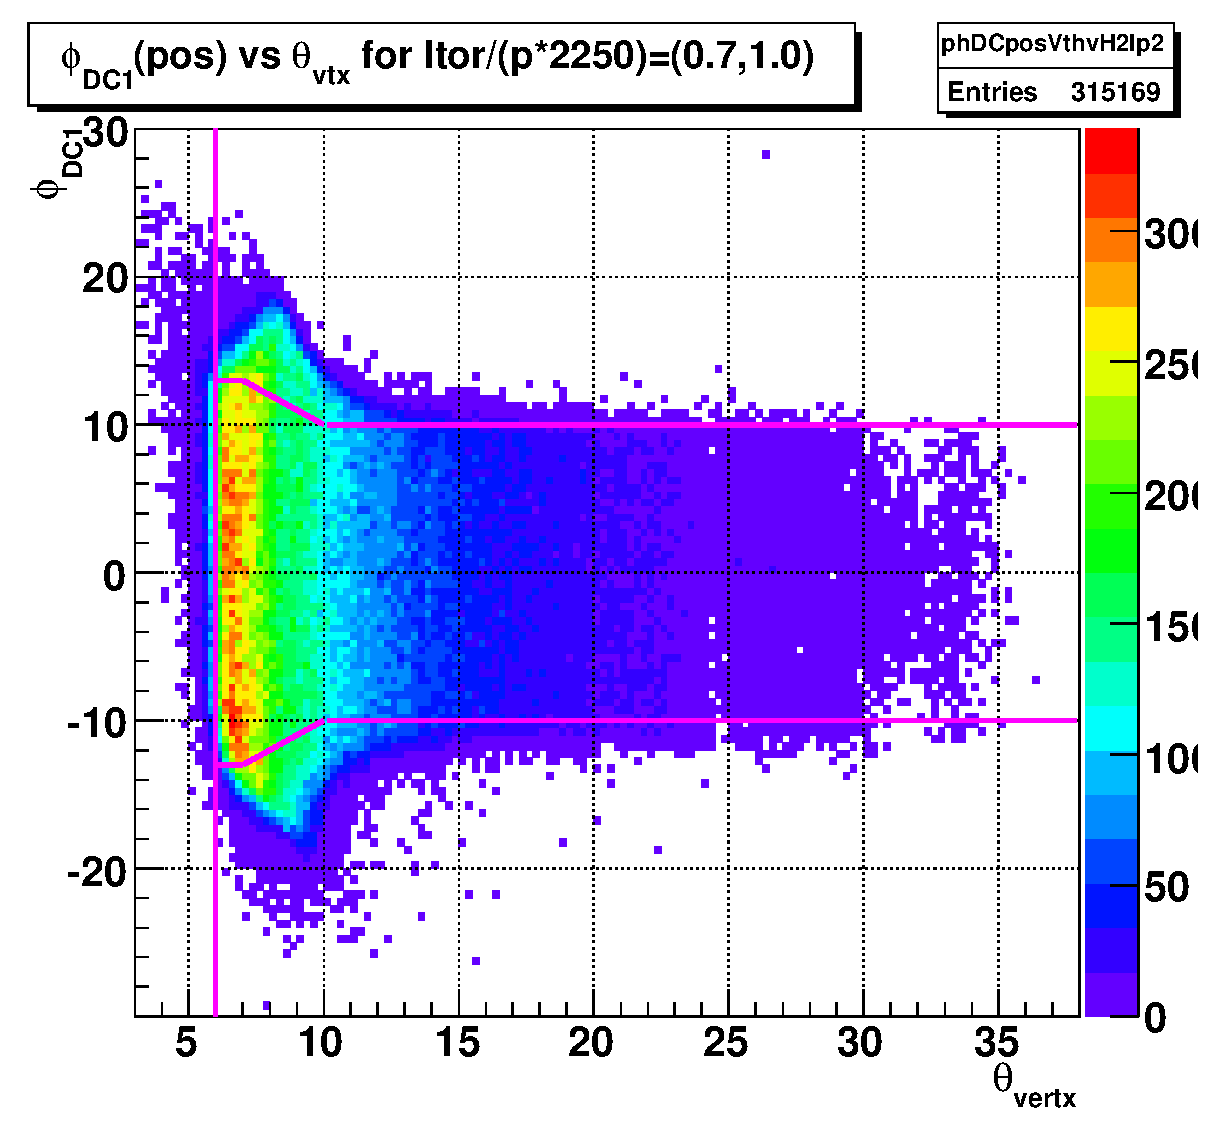
\includegraphics[width=0.9\textwidth]{TexmakerMyFinTh/chap4simul/FigCuts/phDc1PosVsThv_inInvPbins_ExpEb2WdOsiNphNoThCts4Ths.eps} 
%\leavevmode 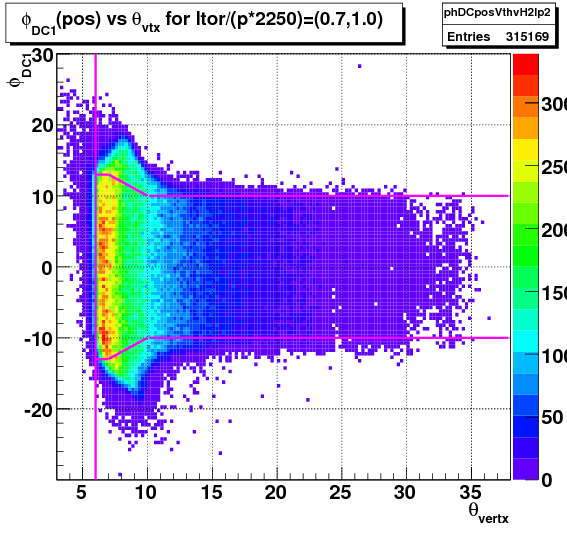
\includegraphics[width=0.9\textwidth]{TexmakerMyFinTh/chap4simul/FigCuts/phDc1PosVsThv_inInvPbins_ExpEb2WdOsiNphNoThCts4Ths} 
%\leavevmode 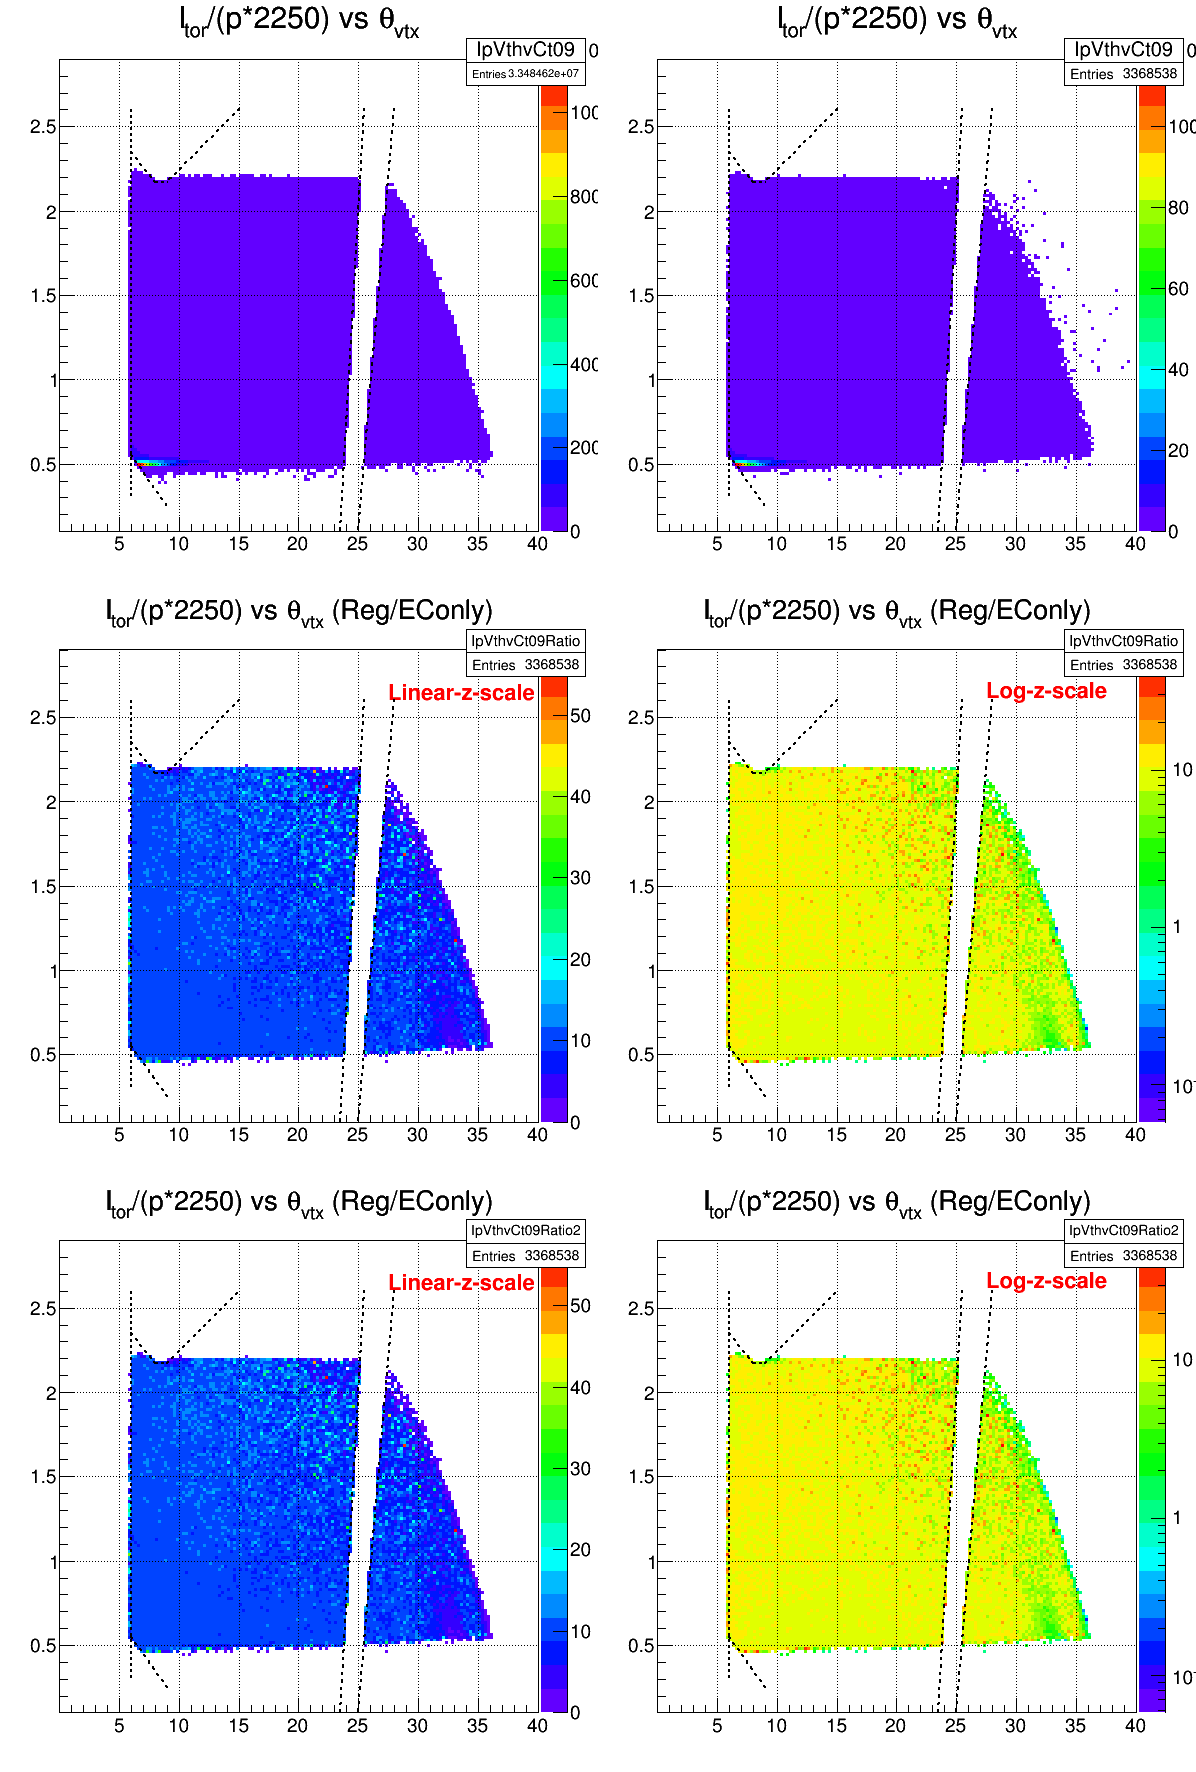
\includegraphics[width=0.9\textwidth]{figuresEG4/NewP2/FidCuts/invMomVsThVtxPass2Ebi1RatioRegByEConlyFidCut09.png}
\leavevmode 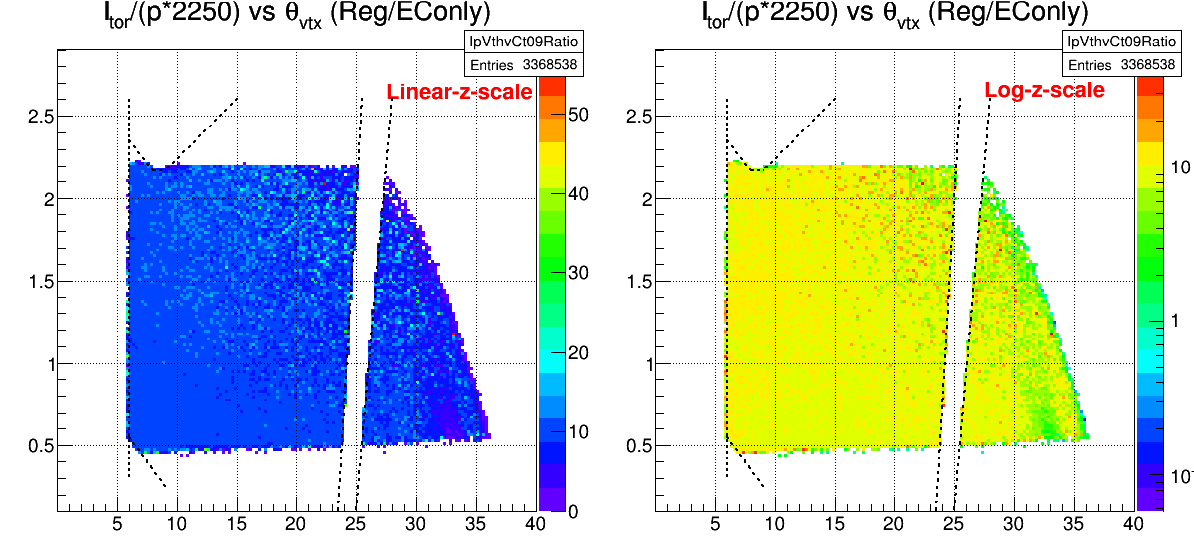
\includegraphics[width=0.9\textwidth]{figuresEG4/NewP2/FidCuts/invMomVsThVtxPass2Ebi1RatioRegByEConlyFidCut09cropped.png}
\caption[Fiducial cuts]{Fiducial cuts determined by comparing the distributions of regular and EC-only {\bf experimental data} as a function of \invP and vertex angle \thvtx. Here, the vertical cut near \thvtx=25 degrees is to avoid the region of low efficiency possibly due to %some dead wires
  dead wires in DC.} %Fiducial cuts
\label{figFidRegVsEC2}
\end{figure}



The third set of cuts came from a %somewhat similar
comparison %but this time 
between the experimental and the corresponding simulated data as shown in the Fig. \ref{figFidExpVsSim}. 
%The ratio of their distributions in a two dimensional space defined in terms of two variables \thvtx and the torus current normalized inverse momentum (i.e. $ I_{torus}/(2250 p)$. In one case, the ratio was taken between the regular experimental data and the "EC-only" experimental data (with CC-signal not required in the event trigger) (see Fig. \ref{figRegByEConly}) and in the other case, the ratio was of the experimental deuteron data (after background subtraction) to the simulated deuteron data (see Fig. \ref{figangCts2}). From these comparisons, some of the regions that showed big CC-inefficiencies or big discrepancies between data and simulation were selected and removed from the fiducial region %defined in terms of some more cuts 
as indicated by various straight lines in the two plots.



\begin{figure}[H]%[h] %ht, htpb (p - float, b = bottom, h=? t = top)
\centering
%\leavevmode 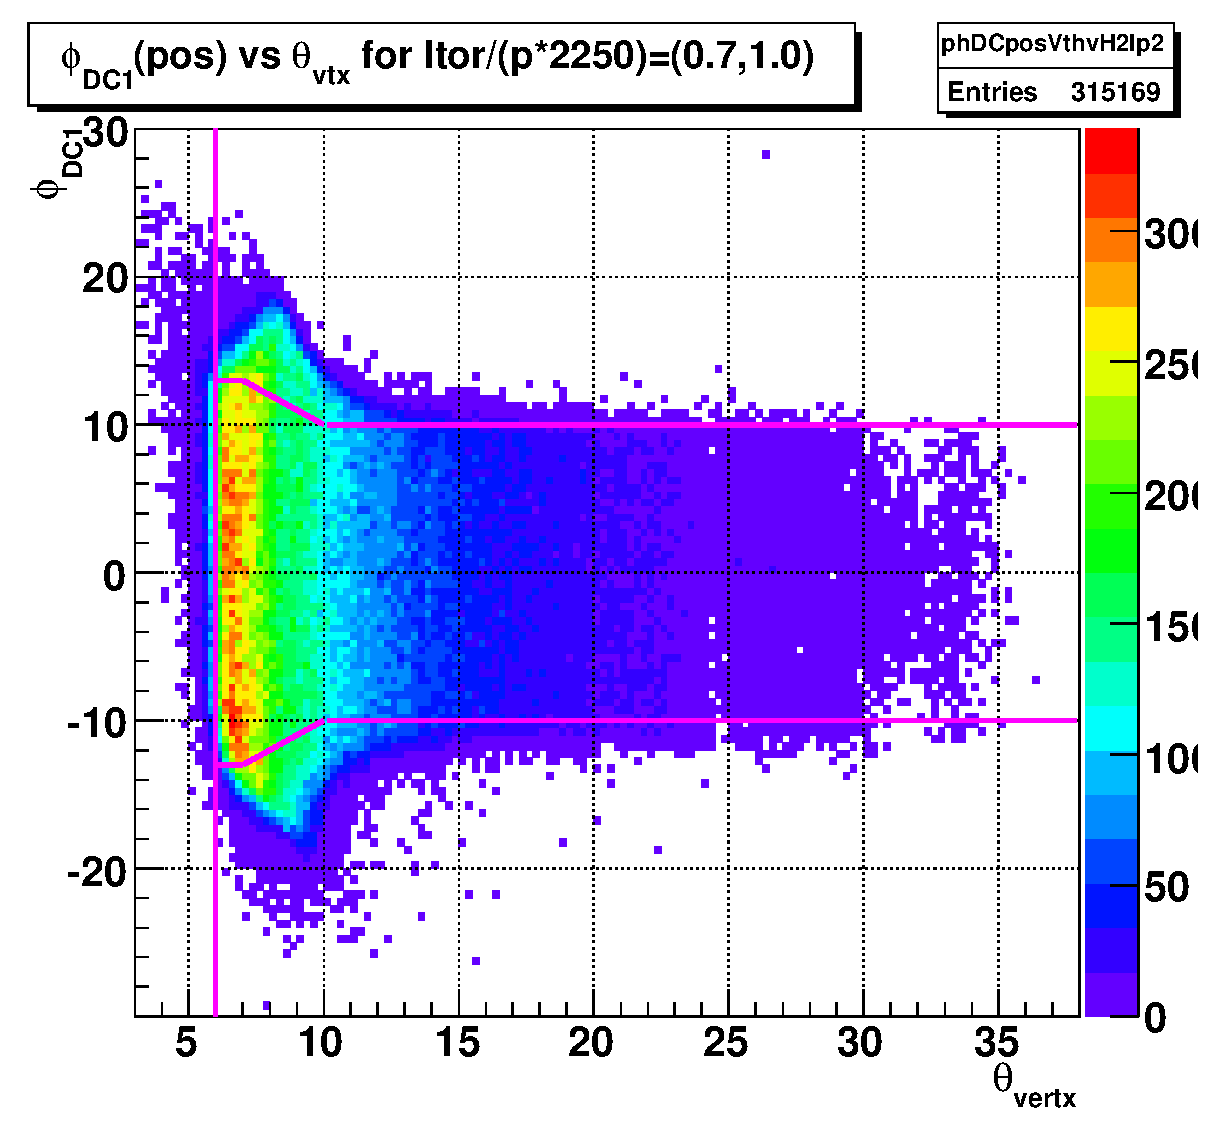
\includegraphics[width=0.9\textwidth]{TexmakerMyFinTh/chap4simul/FigCuts/phDc1PosVsThv_inInvPbins_ExpEb2WdOsiNphNoThCts4Ths.eps} 
%\leavevmode 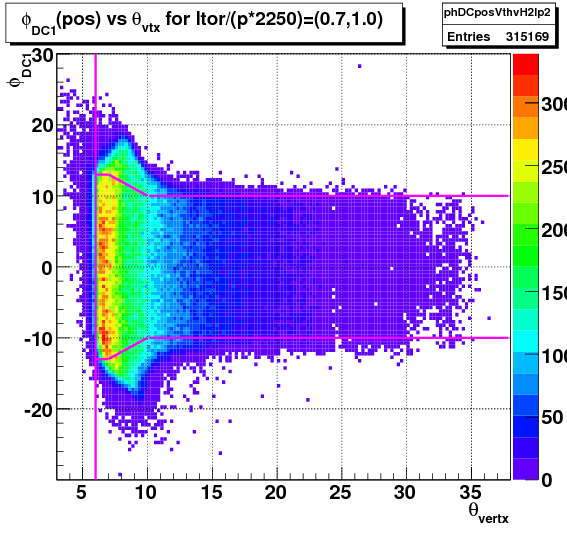
\includegraphics[width=0.9\textwidth]{TexmakerMyFinTh/chap4simul/FigCuts/phDc1PosVsThv_inInvPbins_ExpEb2WdOsiNphNoThCts4Ths} 
%\leavevmode 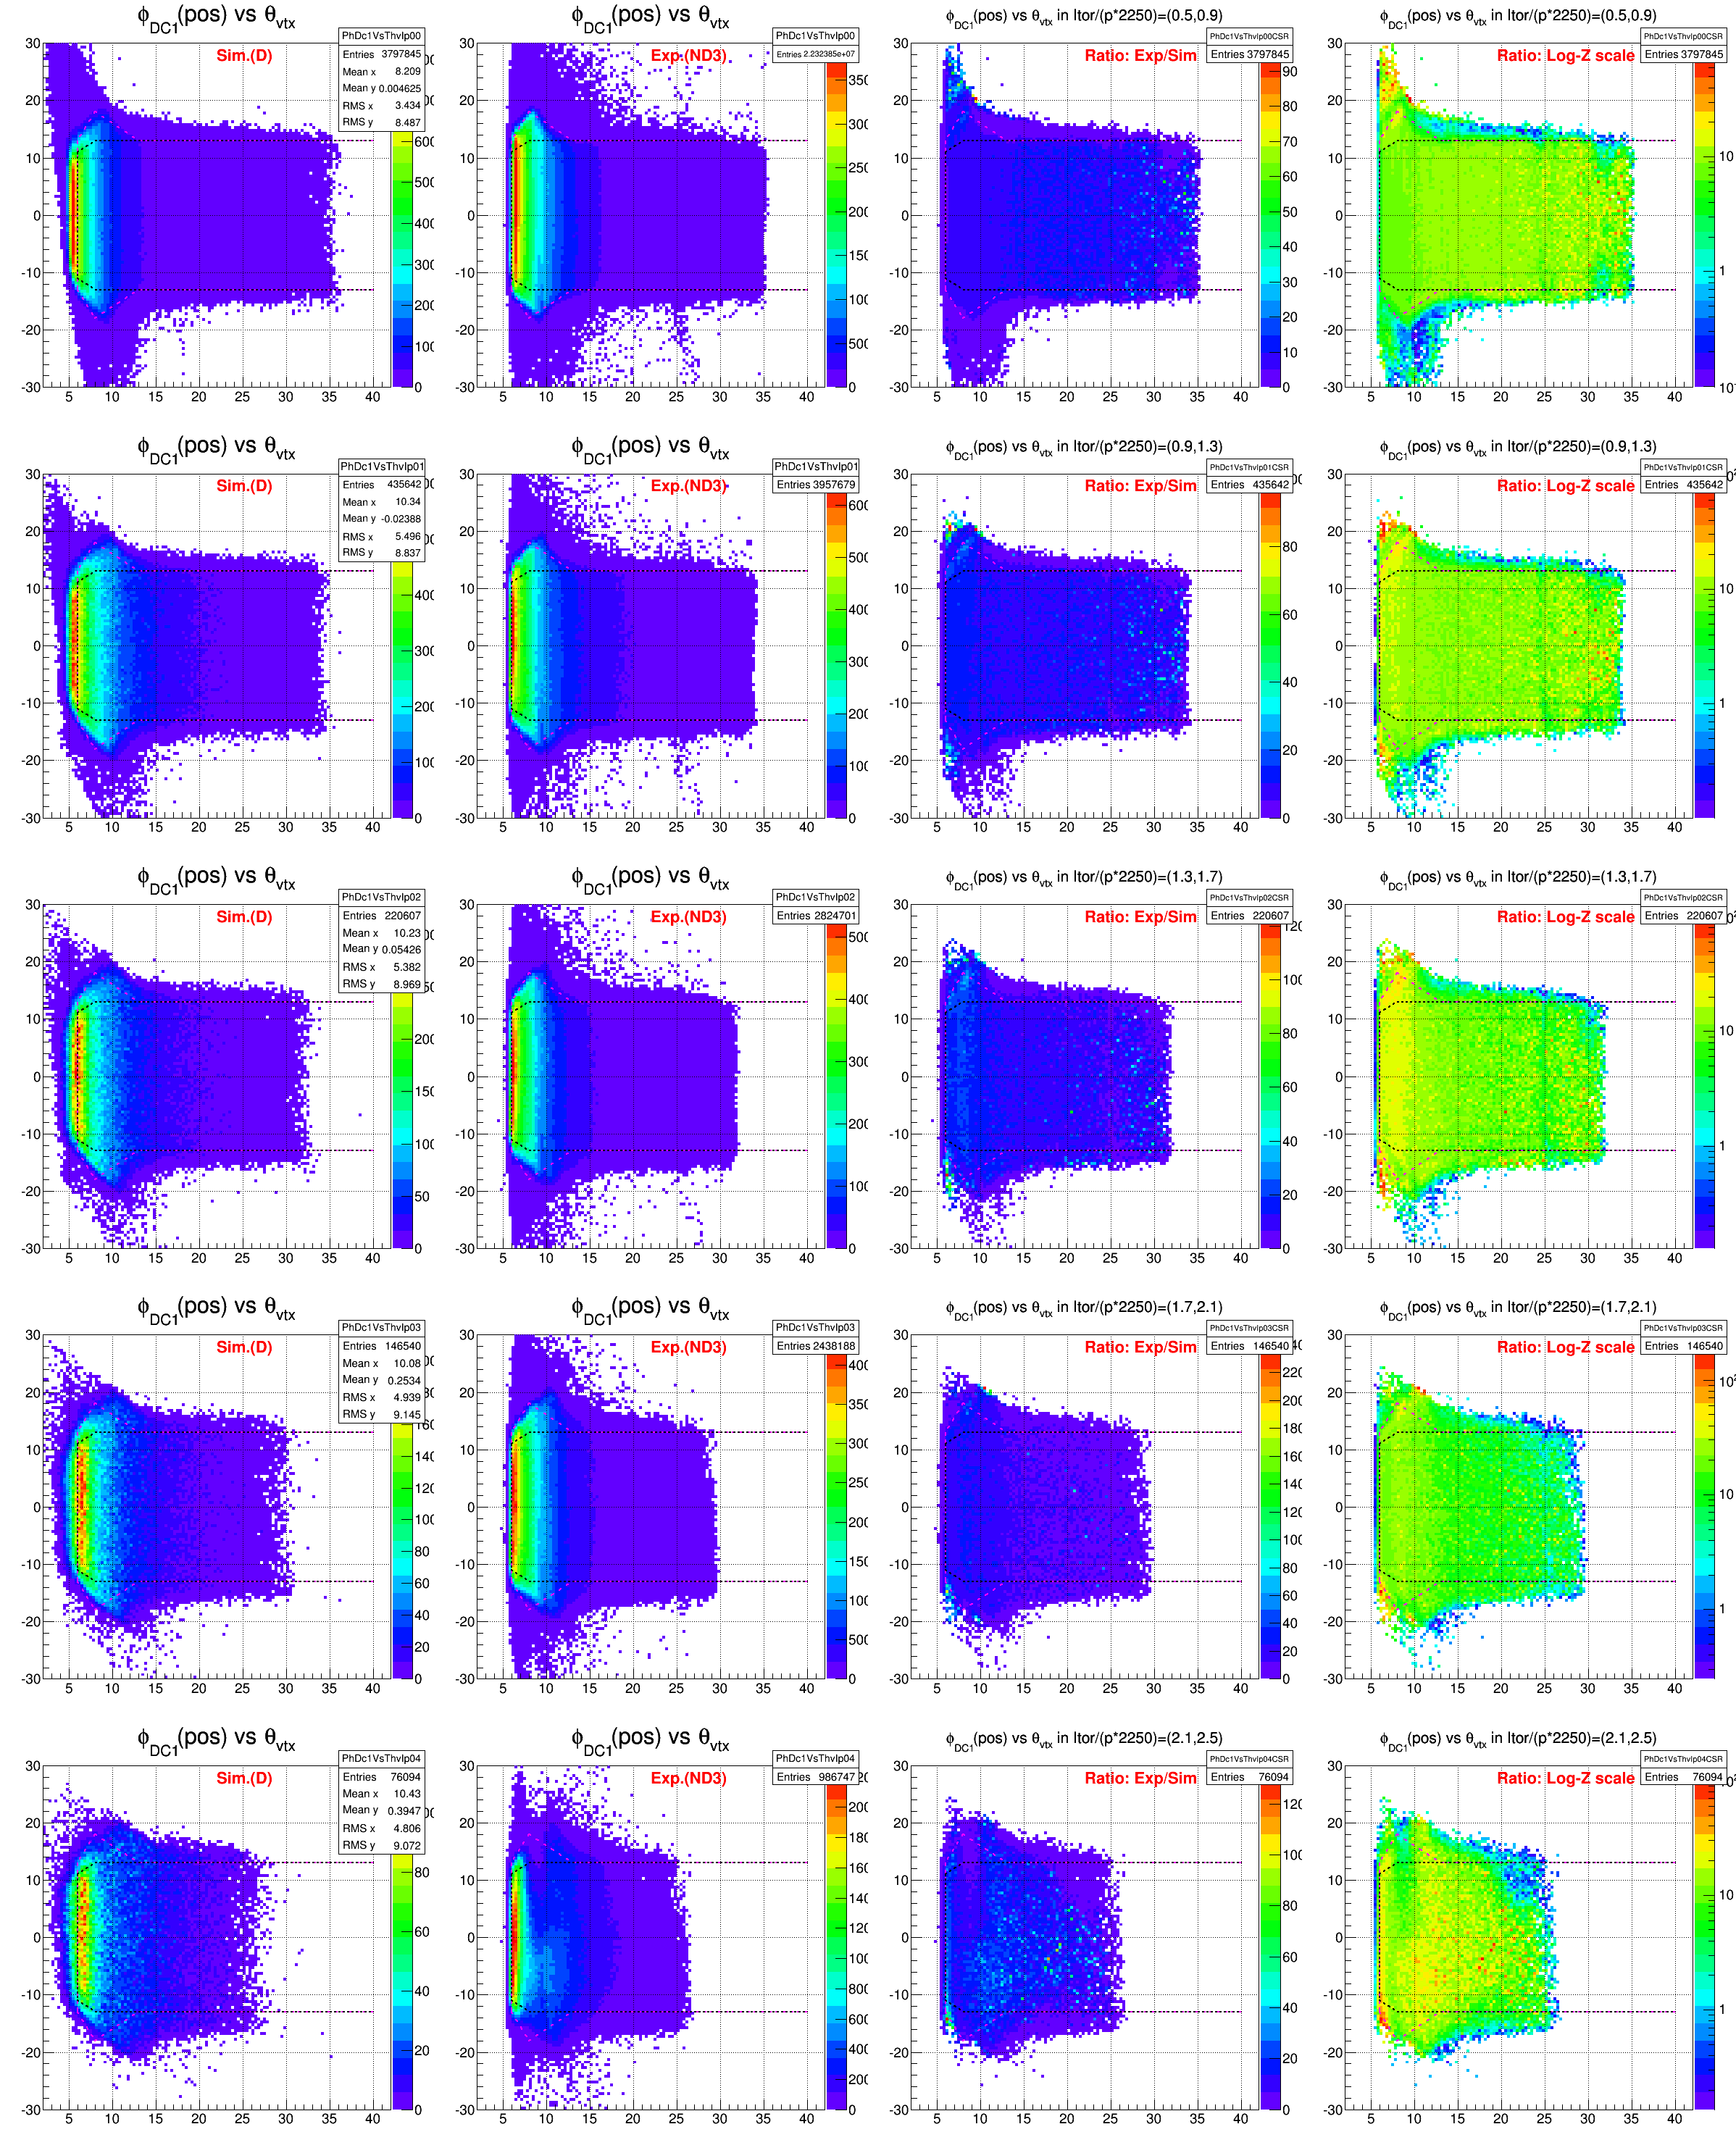
\includegraphics[width=0.98\textwidth]{figuresEG4/NewP2/FidCuts/fidCutPlotsSet2_Eb2_RatioBigger.png}
\leavevmode 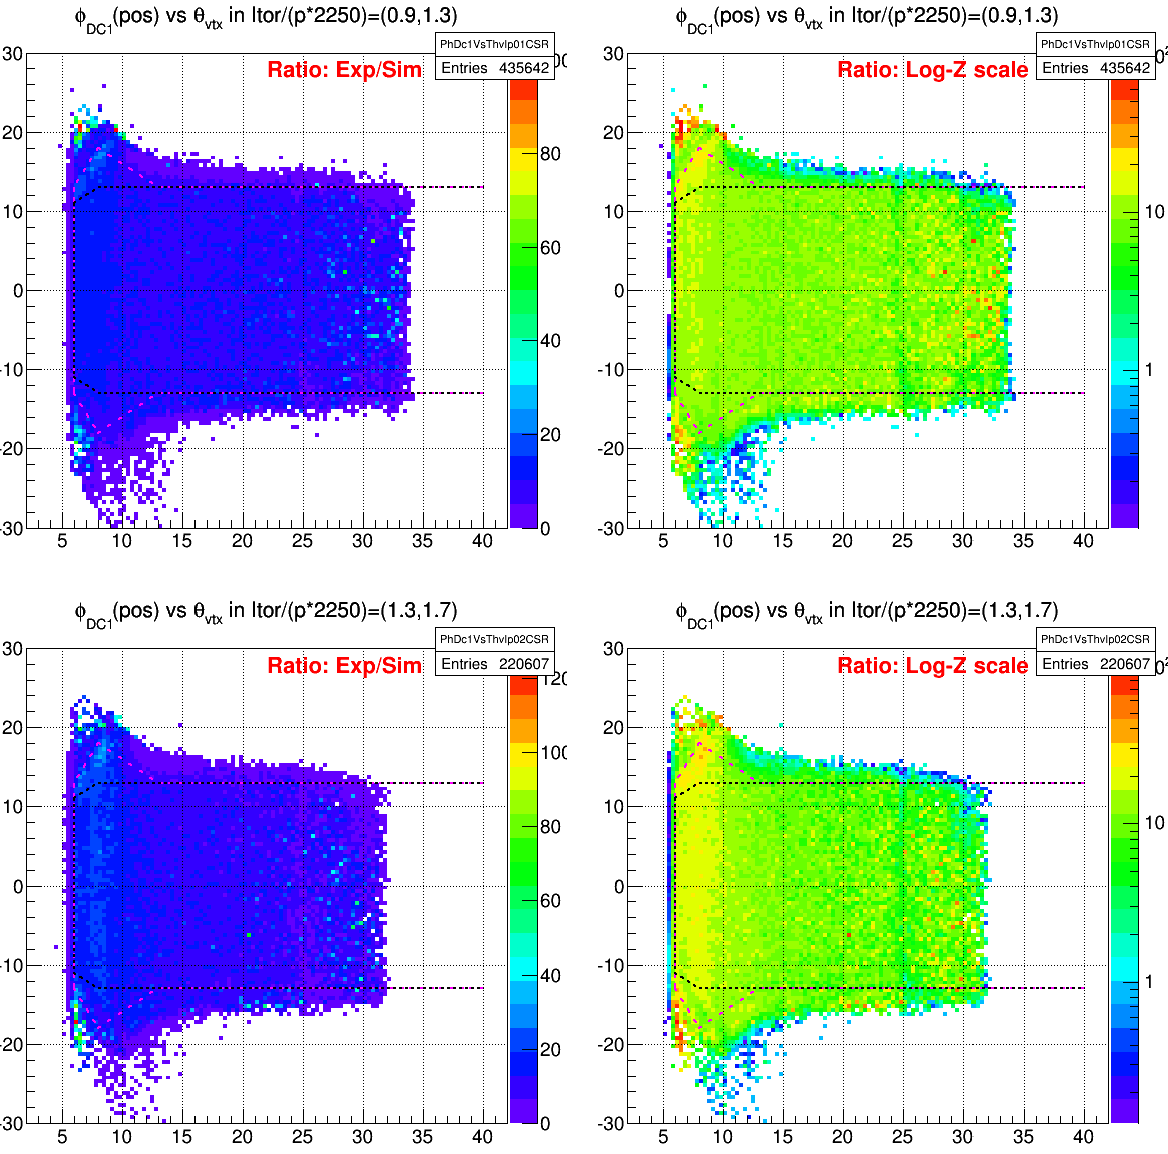
\includegraphics[width=0.98\textwidth]{figuresEG4/NewP2/FidCuts/fidCutPlotsSet2_Eb2_RatioBiggerCroppedIpBins0n1.png}
\caption[Fiducial cuts ]{Distribution (in two of six bins of $I_{torus}/(2250 p)$) of %{\bf experimental} and {\bf simulated} data ( for 2.0 GeV) and their ratios 
ratios of {\bf experimental} and {\bf simulated} data ( for 2.0 GeV) (both in linear and log-z scales) as a function of vertex angle \th and azimuthal angle $\phi_{DC1}$ as measured by the track position at the first drift chamber layer (angles in degrees). The dotted lines indicate the fiducial cuts for accepting good electrons. %\textcolor{red}{SEK: Do you have the analogous plot for simulation? Include \\ Make magenta lines thicker. } %Comment out eventually
} %Fiducial cuts}
\label{figFidExpVsSim}
\end{figure}


%> 1) Fiducial cuts (Very short)   %Dr. Kuhn's comment on Jlab email dated November 3, 2013 3:45 pm  (title Re: "Complete" Thesis)
%
%p. 116: We used the polar angle at the vertex NOT because it isn't affected by the target magnetic field (it most certainly is), but because the acceptance is defined by the range in scattering angle (as you showed earlier, dOm = sintheta dtheta dphi). For the same reason, we SHOULD have chosen phi at the vertex, as well; however, since the effect of the target field on phi is just a constant offset (rotation around the z-axis), the range phi_max - phi_min is the same at DC1 as at the vertex, giving the same acceptance. We chose DC1 because that's what actually limits the phi acceptance. As you understand, this section is not yet complete. You need to explain that we use the amount of bending (Itor/p*2250) as a 3rd variable, since E'=p is the third variable the determines the acceptance, but the amount of bending has direct correlation to where on the CC a track ends (i.e., the phi range). (You should move the corresponding explanation of ip up from p.122).                      You should also show a couple more plots with different Itor/p*2250 as well as a couple of plots for the simulation to convince the reader that our choices are robust.                   Figs. 51a and 51b should be given a full width each since they have a lot of information and are hard to read otherwise (make them two different figures). I also am confused about your explanation for Fig. 51a):                  I seem to remember that we divided ND3 for standard trigger by ND3 for EC only trigger;  dividing ND3 data by D simulation seems to make little sense. Please check!

Lastly, further sets of cuts were developed based on the distribution of average number of photo electrons (nphe) as recorded by the Cerenkov Counter (CC) (see Fig. \ref{figFidAvgNph}).

\begin{comment}
\begin{figure}[H]%[h] %ht, htpb (p - float, b = bottom, h=? t = top)
\centering
\leavevmode 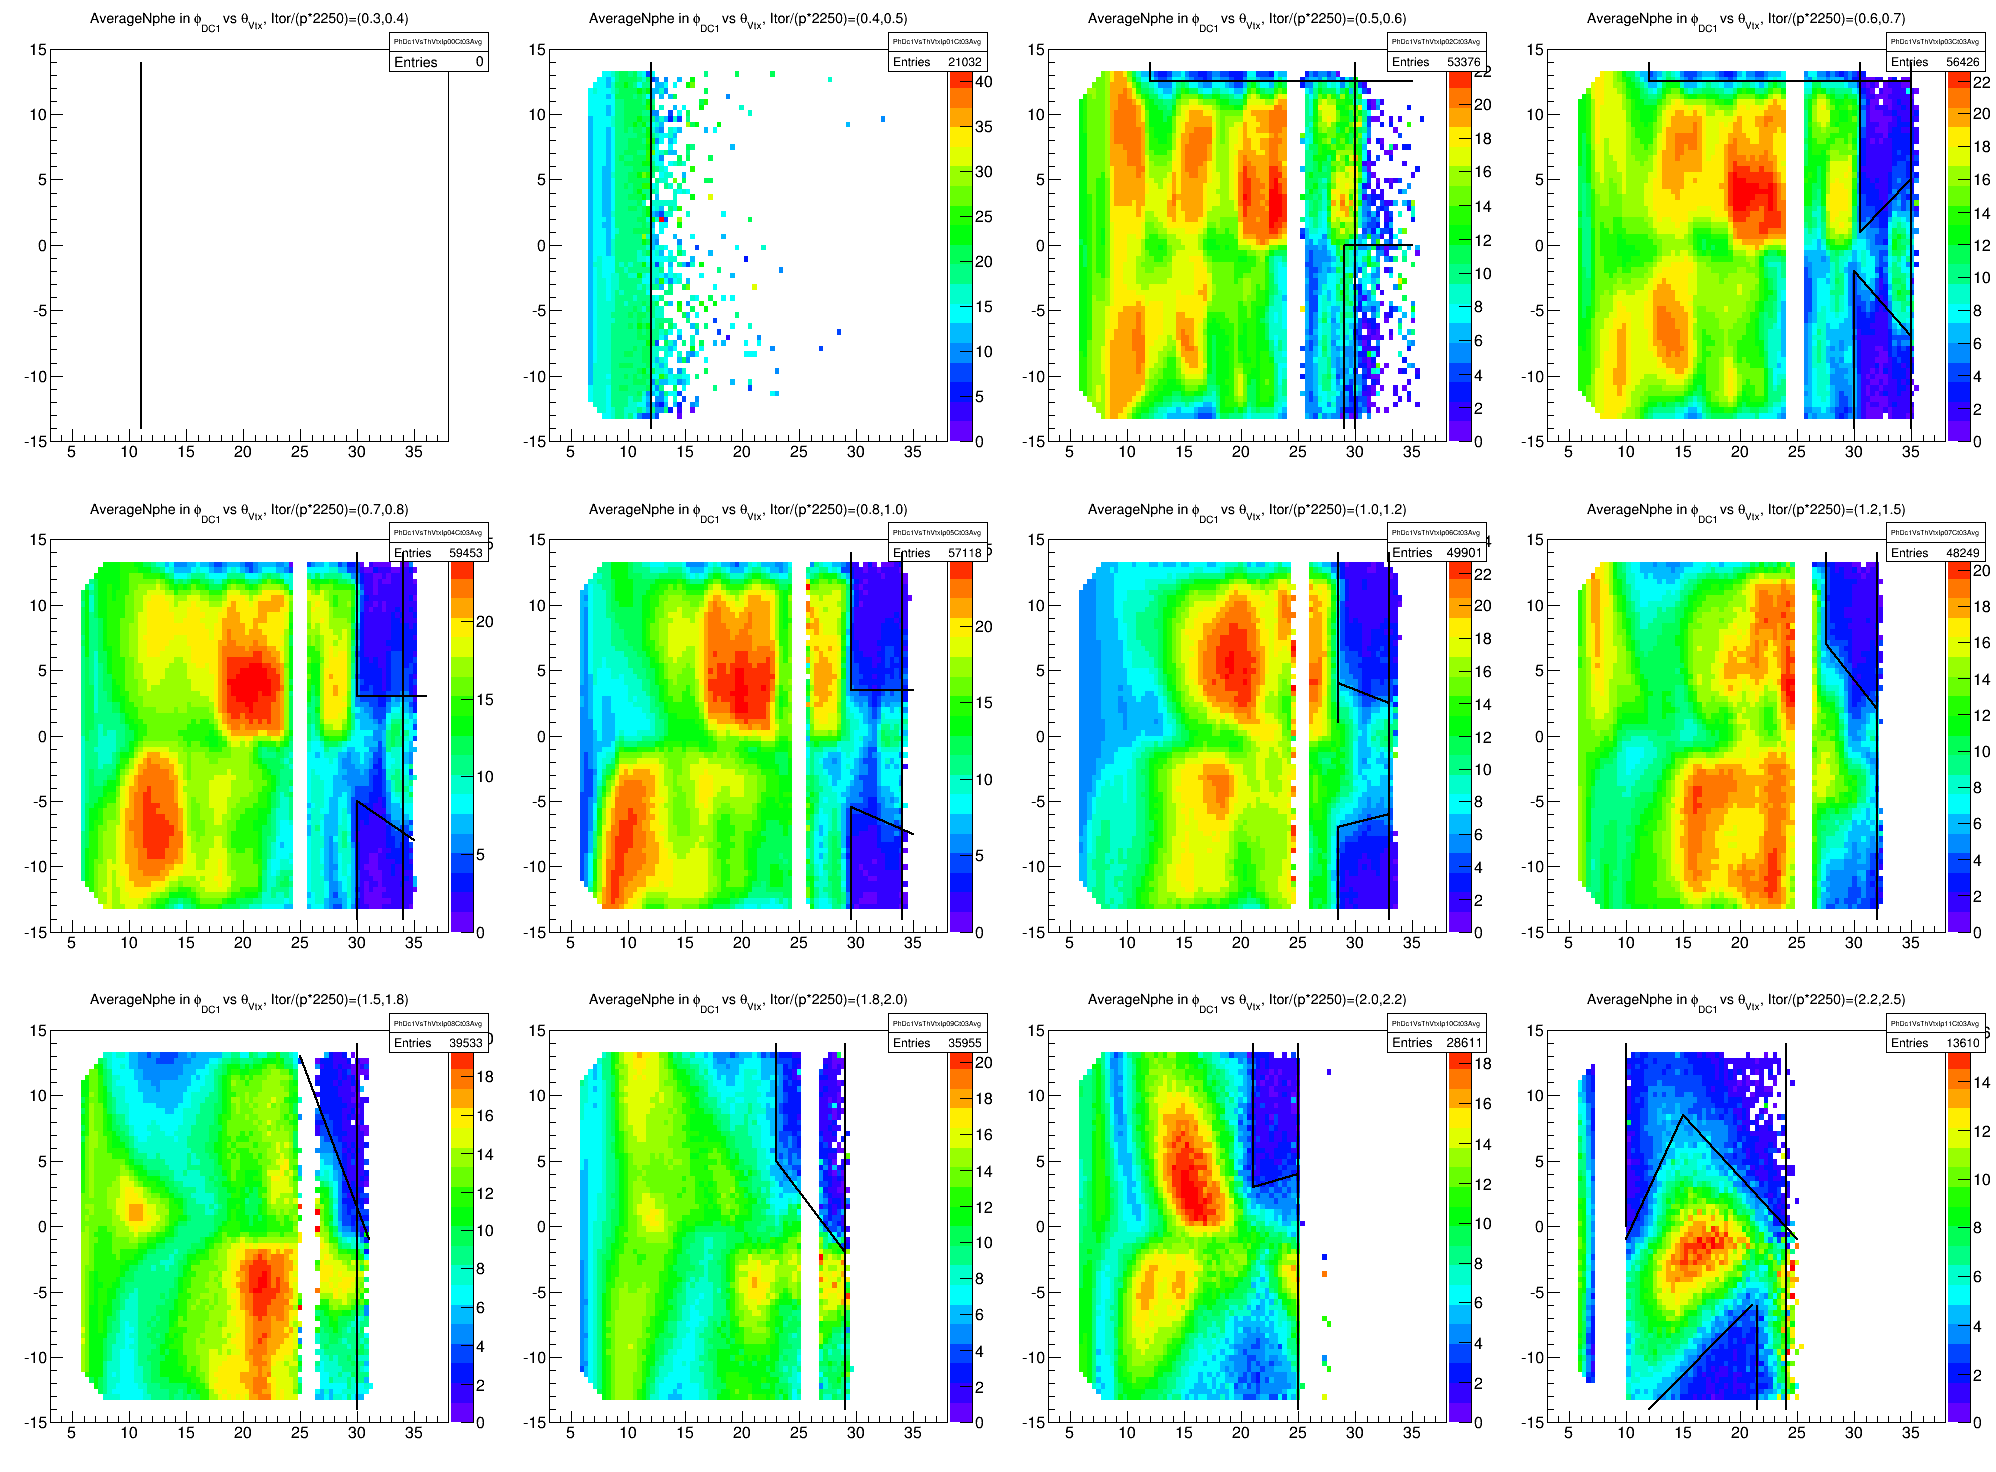
\includegraphics[width=1.1\textwidth]{figuresEG4/NewP2/FidCuts/moreFiducialCutsMoreInversePBinsEbi2.png}
\caption[Fiducial cuts ]{}
\label{figFidAvgNph}
\end{figure}
\end{comment}


\begin{figure}[H]%[h] %ht, htpb (p - float, b = bottom, h=? t = top)
\centering
\leavevmode 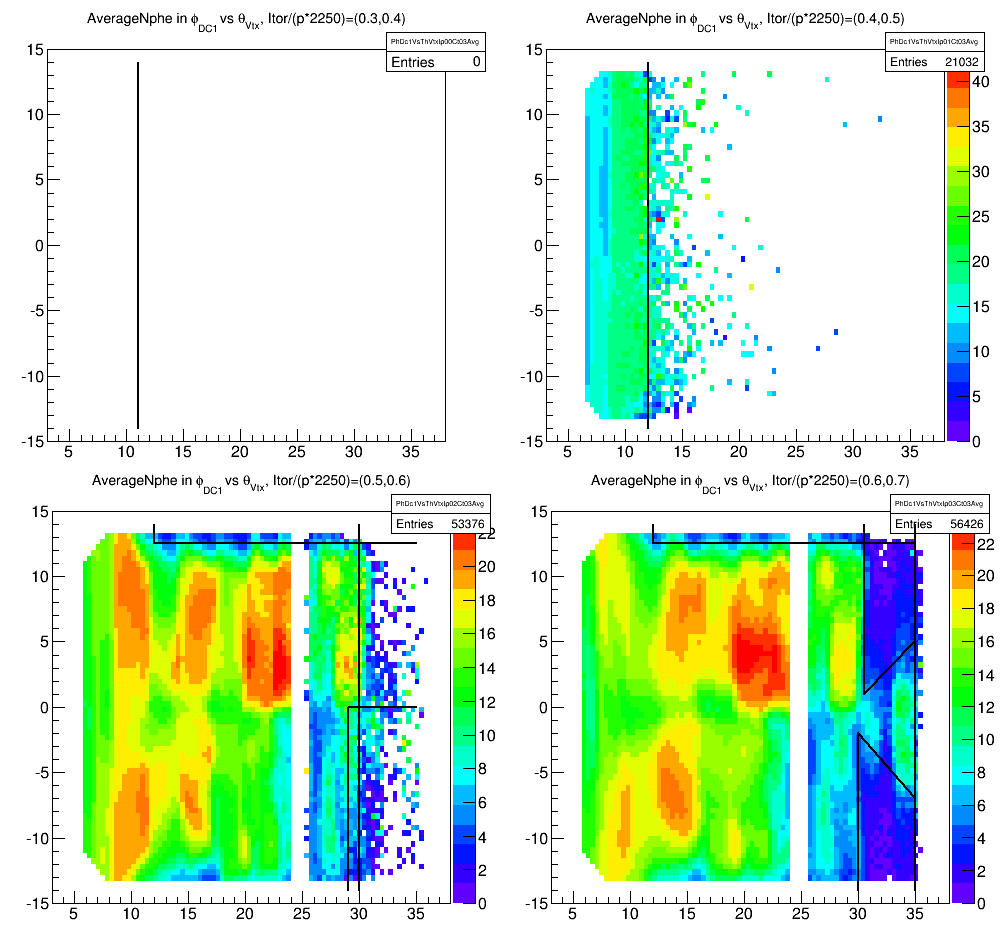
\includegraphics[width=1.1\textwidth]{figuresEG4/NewP2/FidCuts/moreFiducialCutsMoreInversePBinsEbi2first4Bins.png}
\caption[Fiducial cuts (first 4 bins)]{Average Nphe distributions as a function of $\phi_{DC1}$ (along Y-axis) and $\theta_{vtx}$ (along X-axis) in first four bins of $\frac{I_{tor}}{p \cdot 2250}$. The black lines show the cuts that reject the very low CC-inefficiency regions.}
\label{figFidAvgNph1}
\end{figure}


\begin{figure}[H]%[h] %ht, htpb (p - float, b = bottom, h=? t = top)
\centering
\leavevmode 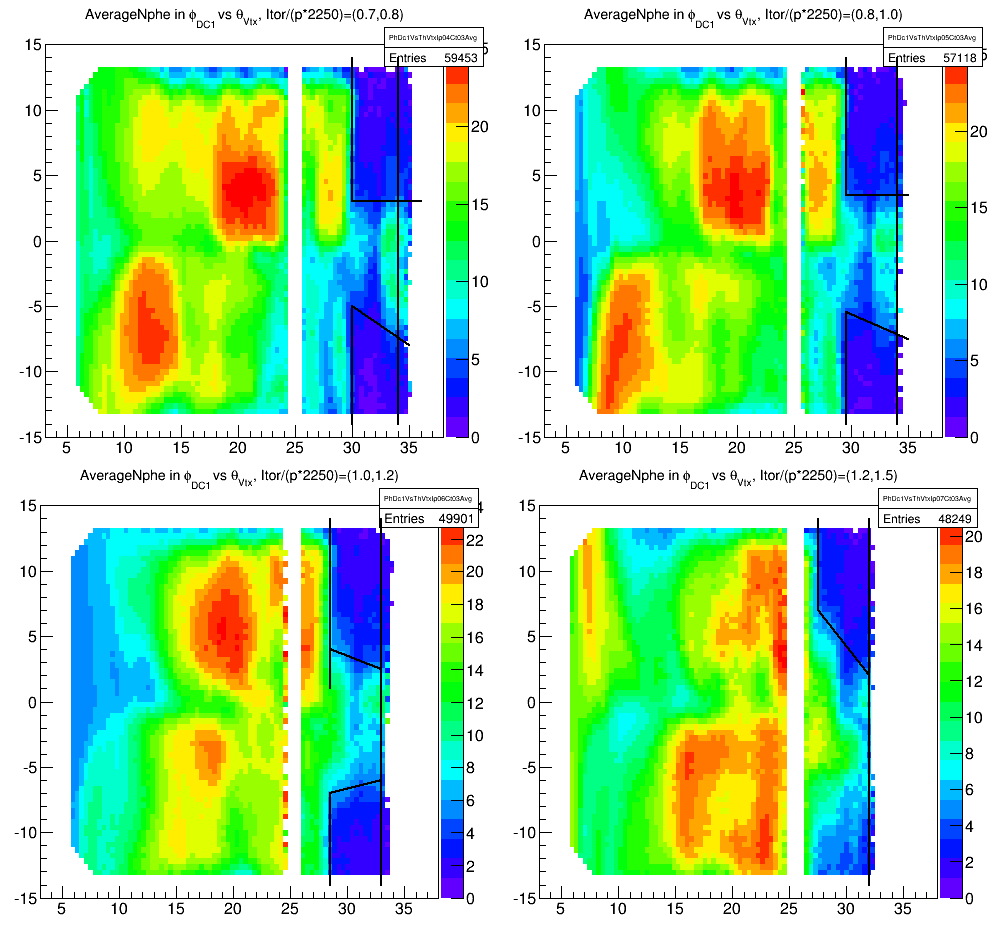
\includegraphics[width=1.1\textwidth]{figuresEG4/NewP2/FidCuts/moreFiducialCutsMoreInversePBinsEbi2next4Bins.png}
\caption[Fiducial cuts (next 4 bins)]{Average Nphe distributions as a function of $\phi_{DC1}$ (along Y-axis) and $\theta_{vtx}$ (along X-axis) in next four bins of $\frac{I_{tor}}{p \cdot 2250}$. The black lines show the cuts that reject the very low CC-inefficiency regions.}
\label{figFidAvgNph1}
\end{figure}


\begin{figure}[H]%[h] %ht, htpb (p - float, b = bottom, h=? t = top)
\centering
\leavevmode 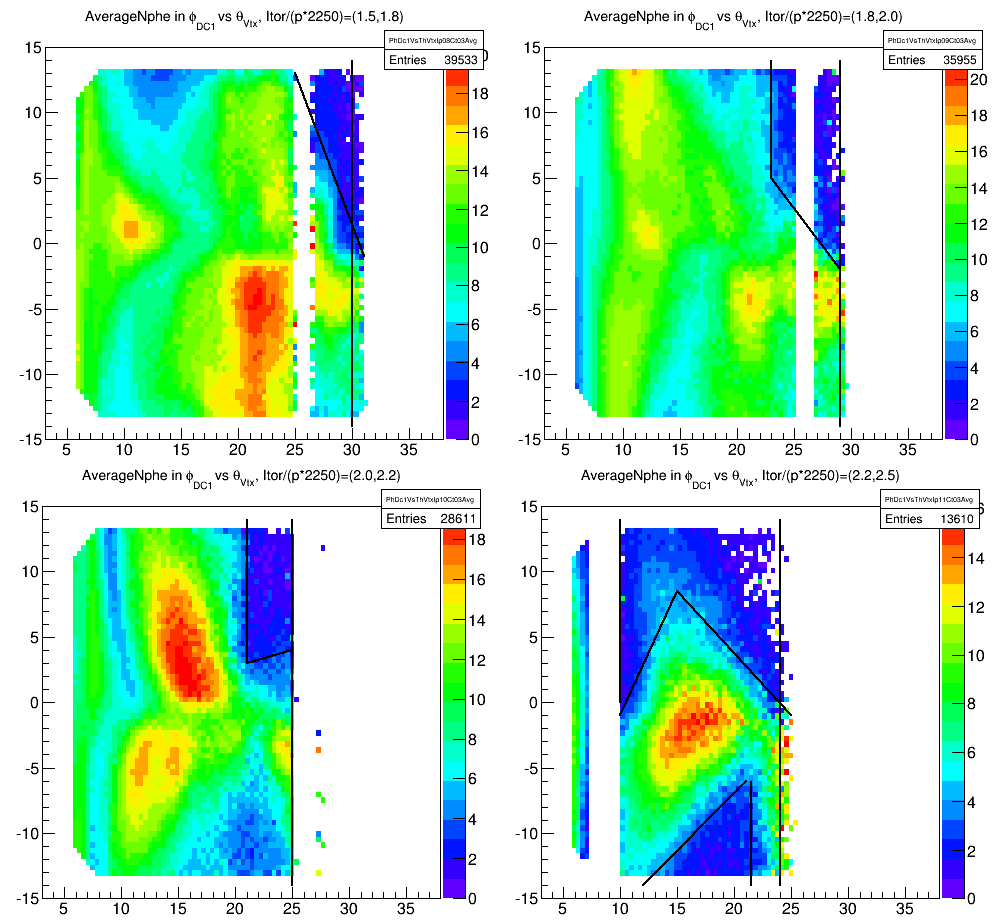
\includegraphics[width=1.1\textwidth]{figuresEG4/NewP2/FidCuts/moreFiducialCutsMoreInversePBinsEbi2last4Bins.png}
\caption[Fiducial cuts (last 4 bins)]{Average Nphe  distributions as a function of $\phi_{DC1}$ (along Y-axis) and $\theta_{vtx}$ (along X-axis) in last four bins of $\frac{I_{tor}}{p \cdot 2250}$. The black lines show the cuts that reject the very low CC-inefficiency regions.}
\label{figFidAvgNph1}
\end{figure}
